%%%%%%%%%%%%%%%%%%%%%%%% themes and packages %%%%%%%%%%%%%%%%%%%%%%%%%
\documentclass[aspectratio=1610]{beamer}

% colors
% taken from https://identity.stanford.edu/overview/color
\definecolor{cardinal}{HTML}{8C1515}
\definecolor{sandstone}{HTML}{D2C295}
\definecolor{westar}{HTML}{DAD7CB}

\mode<presentation>
% basics, courtesy of the CambridgeUS theme
\useoutertheme{infolines}
\useinnertheme[shadow=false]{rounded}
\setbeamerfont{block title}{size={}}
% custom colors
\usecolortheme{beaver}
\setbeamercolor{frametitle}{fg=cardinal,bg=sandstone!20}
\setbeamercolor{local structure}{fg=black}
\setbeamercolor{palette primary}{fg=cardinal,bg=sandstone}
\setbeamercolor{palette secondary}{fg=cardinal,bg=westar}
\setbeamercolor{palette tertiary}{fg=white,bg=cardinal}
\setbeamercolor{titlelike}{fg=cardinal,bg=sandstone!20}
% kill certain unprofessional elements
\setbeamertemplate{navigation symbols}{}
\setbeamertemplate{bibliography item}{}
\setbeamertemplate{section in toc}%
{\inserttocsectionnumber.~\inserttocsection}
\setbeamertemplate{subsection in toc}%
{\hspace{1em}$\bullet$~\inserttocsubsection\par}
\setbeamertemplate{itemize items}{$\bullet$}

% plain and definition theorem styles in sandstone
\makeatletter
\def\th@plain{
  \normalfont
  \setbeamercolor{block title example}{bg=sandstone,fg=white}
  \setbeamercolor{block body example}{bg=sandstone!20,fg=black}
  \def\inserttheoremblockenv{exampleblock}
}
\theoremstyle{plain}
\newtheorem{conjecture}{Conjecture}
\newtheorem{proposition}{Proposition}

\def\th@definition{
  \normalfont
  \setbeamercolor{block title example}{bg=sandstone,fg=white}
  \setbeamercolor{block body example}{bg=sandstone!20,fg=black}
  \def\inserttheoremblockenv{exampleblock}
}
\theoremstyle{definition}

% highlight theorem style in cardinal
\makeatletter
\def\th@highlight{
  \normalfont
  \setbeamercolor{block title example}{bg=cardinal,fg=white}
  \setbeamercolor{block body example}{bg=cardinal!20,fg=black}
  \def\inserttheoremblockenv{exampleblock}
}
\makeatother
\theoremstyle{highlight}
\newtheorem{hconjecture}{Conjecture}
\newtheorem{hcorollary}{Corollary}
\newtheorem{htheorem}{Theorem}
\newtheorem{question}{Question}
\newtheorem{answer}{Answer}


\usepackage{amssymb}
\usepackage{graphicx}
\usepackage{color}
\usepackage{hyperref}
\usepackage{enumerate}
\usepackage{tikz}

\newcommand{\C}{\mathbb{C}}
\newcommand{\F}{\mathbb{F}}
\newcommand{\N}{\mathbb{N}}
\renewcommand{\O}{\mathcal{O}}
\renewcommand{\P}{\mathbb{P}}
\newcommand{\Q}{\mathbb{Q}}
\newcommand{\U}{\mathcal{U}}
\newcommand{\Z}{\mathbb{Z}}

\renewcommand{\l}{\lambda}
\newcommand{\s}{\sigma}
\renewcommand{\t}{\tau}

\newcommand{\es}{\emptyset}
\newcommand{\ol}{\overline}

\newcommand{\gal}{\mathrm{Gal}}
\newcommand{\preper}{\mathrm{PrePer}}
\newcommand{\res}{\mathrm{Res}}

\newcommand{\set}[1]{\left\{#1\right\}}
\newcommand{\tup}[1]{\left<#1\right>}


%%%%%%%%%%%%%%%%%%%%%%%%%%% title and toc %%%%%%%%%%%%%%%%%%%%%%%%%%%%

\title[Quadratic periodic points]%
{On quadratic periodic points of quadratic polynomials}

\author{Zhiming Wang and Robin Zhang} % Your name
\institute[Stanford]
{
Stanford University\\
\medskip
\textit{zmwang@stanford.edu}\\
\textit{robinz16@stanford.edu}
}
\date{August 28, 2014}

\begin{document}

\begin{frame}
  \titlepage
\end{frame}

\begin{frame}
  \frametitle{Overview}
  \tableofcontents
\end{frame}

%%%%%%%%%%%%%%%%%%%%%%%%%%%%%%%% body %%%%%%%%%%%%%%%%%%%%%%%%%%%%%%%%

\fontsize{8pt}{9.6}\selectfont

\section{Introduction}

\begin{frame}
  \frametitle{Introduction}
  \begin{minipage}{\textwidth}
    \begin{columns}
      \begin{column}{0.8\textwidth}
        \textbf{Goal: Study the periodic points, or cycles, of
          quadratic polynomials $\phi$.}

        \[
        \phi(z) = a_2 z^2 + a_1 z + a_0
        \xrightarrow{\text{linear conjugation}}
        \phi_c(z) = z^2 + c
        \]

        preserves size of orbits; reduce to studying cycles of
        $\phi_c(z)$.

      \end{column}

      \begin{column}{0.2\textwidth}
        \center
        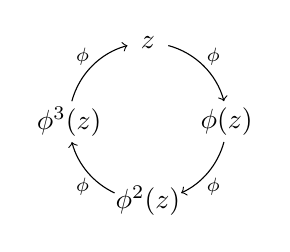
\begin{tikzpicture}
          \node at (1,2) {$z$};
          \node at (2,1) {$\phi(z)$};
          \node at (1,0) {$\phi^2(z)$};
          \node at (0,1) {$\phi^3(z)$};
          \draw [->] (1.25882,1.96593) arc
          [radius=1, start angle=75, end angle=15];
          \draw [->] (1.96593,0.74118) arc
          [radius=1, start angle=-15, end angle=-65];
          \draw [->] (0.57738,0.09369) arc
          [radius=1, start angle=-115, end angle=-165];
          \draw [->] (0.03407,1.25882) arc
          [radius=1, start angle=165, end angle=105];
          \node at (1.83,1.83) {\scriptsize$\phi$};
          \node at (1.83,0.17) {\scriptsize$\phi$};
          \node at (0.17,0.17) {\scriptsize$\phi$};
          \node at (0.17,1.83) {\scriptsize$\phi$};
        \end{tikzpicture}

        Example of a 4-cycle.
      \end{column}
    \end{columns}
  \end{minipage}

  \pause

  \begin{minipage}{\textwidth}
    \textbf{The model:}

    Periodic points of period $N$ are characterized by $\phi_c^N(z) -
    z = 0$. By the M\"obius inversion formula, we have
    \[
    \phi_c^N(z) - z = \prod_{d|N} \Phi_d(z, c),
    \]
    where
    \[
    \Phi_d(z, c) = \prod_{m|d}(\phi_c^m(z) - z)^{\mu(d/m)}.
    \]

    \pause

    \textbf{Periodic points of exact period $N$ are characterized by
      $\Phi_N(z, c)$.}

    Let $C_1(N)$ be the algebraic curve defined by $\Phi_N(z, c)$.

    Let $C_0(N)$ be the quotient curve of $C_1(N)$ by the automorphism
    $\sigma: (z, c) \mapsto (\phi_c(z), c)$, i.e., the curve obtained
    by identifying points in the same $N$-cycle on $C_1(N)$.
  \end{minipage}
\end{frame}

\subsection{Previous results}

\begin{frame}
  \frametitle{Previous results}
  \begin{theorem}[Morton, Theorem~4 in \cite{MR1665198}]
    There are no finite rational solutions $(z, c)$ of the equation
    $\Phi_4(z, c) = 0$. In other words, there are no quadratic
    polynomials defined over $\Q$ with rational periodic points of
    exact period 4.
  \end{theorem}

  \begin{theorem}[FPS, Theorem~1 in \cite{MR1480542}]
    There are no quadratic polynomials defined over $\Q$ with rational
    periodic points of exact period 5.
  \end{theorem}

  \begin{theorem}[Stoll, Theorem~7 in \cite{MR2465796}]
    Let $J$ be the Jacobian of $C_0(6)$. If the $L$-series $L(J,s)$
    extends to an entire function and satisfies the standard
    functional equation, and if the weak Birch and Swinnerton-Dyer
    conjecture is valid for $J$, then there are no quadratic
    polynomials defined over $\Q$ with rational periodic points of
    exact period 6.
  \end{theorem}
\end{frame}

\subsection{Our question}

\begin{frame}
  \frametitle{Our question}

  Extend the previous results to quadratic cases.

  \pause

  \begin{definition}
    Let $\U$ be the collection of all rational or quadratic elements
    in $\ol{\Q}$, or equivalently,
    \[
    \U = \bigcup_{[K : \Q] = 2}K,
    \]
    where the union is the union of sets, taken over all quadratic
    extensions of $\Q$.
  \end{definition}

  \pause

  \begin{question}
    \label{question}
    How many $c \in \Q$ are there such that $\phi_c(z) = z^2 + c$ has
    periodic points in $\U$ of exact period $N$?
  \end{question}

  \pause

  \begin{answer}
    \begin{itemize}
    \item $N = 4$, infinite (completely understood)!
    \item $N = 5$, finite!
    \item Also some general results.
    \end{itemize}
  \end{answer}
\end{frame}

\section{The quadratic $N = 4$ case}

\begin{frame}
  \frametitle{The quadratic $N = 4$ case}

  \pause

  \begin{proposition}
    For $\phi_c(z) = z^2 + c$, all combinations of $c$ and a
    corresponding 4-cycle $\set{z_1, z_2, z_3, z_4}$ of $\phi_c(z)$
    can be parametrized over $\C$ by
    \begin{equation}
      \label{eq:4-param}
      \begin{gathered}
        c = \frac{1 - 4t^3 - t^6}{4t^2(t^2 - 1)}, \\
        z_1 = \frac{t^4 - t^2 + \sqrt{(t^4 - 1)(t^2 + 2t - 1)}}{2t(t^2
          - 1)},\,
        z_2 = \frac{1 - t^2 + t \sqrt{(t^4 - 1)(t^2 + 2t -
            1)}}{4t^2(t^2 - 1)}, \\
        z_3 = \frac{t^4 - t^2 - \sqrt{(t^4 - 1)(t^2 + 2t - 1)}}{2t(t^2
          - 1)},\,
        z_4 = \frac{1 - t^2 - t \sqrt{(t^4 - 1)(t^2 + 2t -
            1)}}{4t^2(t^2 - 1)},
      \end{gathered}
    \end{equation}
    where $t = z_1 + z_3$.
  \end{proposition}

  \pause

  \begin{lemma}[Panraksa, Theorem~1.5.1 in \cite{MR2982105}]
    \label{lem:z1+z3}
    Let $c \in \Q$, and let $\set{z_1, z_2, z_3, z_4} \subset K$ be a
    4-cycle of $\phi_c(z) = z^2 + c$, where $K$ is a quadratic
    extension to $\Q$. Then $t = z_1 + z_3$ is rational.
  \end{lemma}

  \pause

  \begin{theorem} [Panraksa, Theorem~1.5.2 in \cite{MR2982105}]
    \label{th:all}
    All combinations $(c, \set{z_1, z_2, z_3, z_4})$, where $c \in \Q$
    and $\set{z_1, z_2, z_3, z_4} \subset K$ is a corresponding
    4-cycle of $\phi_c(z) = z^2 + c$ with $K$ being a quadratic
    extension to $\Q$, are given by ranging $t$ over $\Q$ in the
    parametrization (\ref{eq:4-param}).
  \end{theorem}
\end{frame}

\begin{frame}
  \begin{theorem} [Panraksa, Theorem~1.5.2 in \cite{MR2982105}, same
    as before]
    \label{th:all}
    All combinations $(c, \set{z_1, z_2, z_3, z_4})$, where $c \in \Q$
    and $\set{z_1, z_2, z_3, z_4} \subset K$ is a corresponding
    4-cycle of $\phi_c(z) = z^2 + c$ with $K$ being a quadratic
    extension to $\Q$, are given by ranging $t$ over $\Q$ in the
    parametrization
    \begin{equation}
      \begin{gathered}
        c = \frac{1 - 4t^3 - t^6}{4t^2(t^2 - 1)}, \\
        z_1 = \frac{t^4 - t^2 + \sqrt{(t^4 - 1)(t^2 + 2t - 1)}}{2t(t^2
          - 1)},\,
        z_2 = \frac{1 - t^2 + t \sqrt{(t^4 - 1)(t^2 + 2t -
            1)}}{4t^2(t^2 - 1)}, \\
        z_3 = \frac{t^4 - t^2 - \sqrt{(t^4 - 1)(t^2 + 2t - 1)}}{2t(t^2
          - 1)},\,
        z_4 = \frac{1 - t^2 - t \sqrt{(t^4 - 1)(t^2 + 2t -
            1)}}{4t^2(t^2 - 1)},
      \end{gathered}
    \end{equation}
  \end{theorem}

  \pause

  \begin{hcorollary}
    There are infinitely many $c \in \Q$ such that $\phi_c(z) = z^2 +
    c$ has periodic points in $\U$ of exact period 4. Moreover, all
    such $c$ are given by
    \[
    \label{eq:c-param}
    c = \frac{1 - 4t^3 - t^6}{4t^2(t^2 - 1)},
    \]
    where $t \in \Q$.
  \end{hcorollary}

  \pause

  \begin{theorem}
    For each $c \in \Q$, $\phi_c(z) = z^2 + c$ has at most one 4-cycle
    with points in $\U$, i.e., with points defined over a quadratic
    extension to $\Q$.
  \end{theorem}
\end{frame}

\section{The quadratic $N = 5$ case}

\begin{frame}
  \frametitle{The quadratic $N = 5$ case}

  \pause

  (FPS proved that) $C_0(5)$ is birationally equivalent, through a
  series of changes of coordinates, to
  \begin{equation}
    \label{eq:c0(5)}
    y^2 = f(x) = x^6 + 8x^5 + 22x^4 + 22x^3 + 5x^2 + 6x + 1,
  \end{equation}
  where the original $c$ is given in terms of $x$ and $y$ by
  \begin{equation}
    \label{eq:c-in-xy}
    c = \frac{g(x)}{2(P_0(x) - P_1(x) y)}
    = \frac{P_0(x) + P_1(x) y}{h(x)},
  \end{equation}
  where $g, h, P_0, P_1 \in \Z[x]$ are given by
  \begin{equation}
    \label{eq:poly-defs}
    \begin{aligned}
      & g(x) = 8x^6 + 74x^5 + 271x^4 + 452x^3 + 325x^2 + 110x + 64,
      h(x) = 8x^2(x+3)^2,\\
      & P_0(x) = - x^6 - 10x^5 - 46x^4 - 104x^3 - 95x^2 - 24x - 9,
      P_1(x) = x^3 + 6x^2 + 3x - 9.
    \end{aligned}
  \end{equation}

  \pause

  \begin{htheorem}
    There are finitely many $c \in \Q$ such that $\phi_c(z) = z^2 + c$
    has periodic points in $\U$ of exact period 5.
  \end{htheorem}

  \pause

  \begin{hconjecture}
    There are no $c \in \Q$ such that $\phi_c(z) = z^2 + c$ has
    periodic points in $\U$ of exact period 5.
  \end{hconjecture}

  We have plenty of computational evidence, as well as the backing of
  another conjecture (obtained with a completely different approach),
  which we will explain soon!
\end{frame}

\section{General results}

\newcommand{\nd}{\frac{N}{(N, d)}}

\begin{frame}
  \frametitle{General results}

  \pause

  \begin{lemma} [Panraksa, Lemma~2.3.1 in \cite{MR2982105}]
    Let $c \in \Q$, and let $\set{z_1, z_2, z_3, z_4} \subset K$ be a
    4-cycle of $\phi_c(z) = z^2 + c$, where $K$ is a quadratic
    extension to $\Q$. Then exactly one of the following holds:
    \begin{enumerate}[(i)]
    \item $z_3 = \ol{z_1}$;

    \item $\{z_1, z_2, z_3, z_4\} \cap \{\ol{z_1}, \ol{z_2}, \ol{z_3},
      \ol{z_4}\} =\es.$
    \end{enumerate}
  \end{lemma}

  \pause

  \begin{htheorem}
    Let $N \in \N^*$, $c \in \Q$, $K$ be a Galois extension of $\Q$
    with degree $d = [K : \Q]$, and $\set{z_0, \dots, z_{N-1}} \subset
    K$ be an exact $N$-cycle of $\phi_c(z) = z^2 + c$. Then exactly
    one of the following holds:
    \begin{enumerate}[(i)]
    \item $z_{i\nd} = \t(z_0)$ for some $0 \le i \le (N, d)-1$ and
      some nontrivial $\t \in \gal(K/\Q)$;

    \item $\set{z_0, \dots, z_{N-1}} \cap \set{\t(z_0), \dots,
        \t(z_{N-1})} = \es$ for all nontrivial $\t \in \gal(K/\Q)$.
    \end{enumerate}
  \end{htheorem}

  \pause

  \begin{hconjecture}
    \label{cj:galois-conjugate}
    Let $N \in \N^*$, $c \in \Q$, $K$ be a Galois extension of $\Q$
    with degree $d = [K : \Q]$, and $\set{z_0, \dots, z_{N-1}} \subset
    K$ be an exact $N$-cycle of $\phi_c(z) = z^2 + c$. Then $z_{i\nd}
    = \t(z_0)$ for some $0 \le i \le (N, d)-1$ and some nontrivial $\t
    \in \gal(K/\Q)$.
  \end{hconjecture}
\end{frame}

\begin{frame}
  \begin{hconjecture}[Same as before]
    \label{cj:galois-conjugate}
    Let $N \in \N^*$, $c \in \Q$, $K$ be a Galois extension of $\Q$
    with degree $d = [K : \Q]$, and $\set{z_0, \dots, z_{N-1}} \subset
    K$ be an exact $N$-cycle of $\phi_c(z) = z^2 + c$. Then $z_{i\nd}
    = \t(z_0)$ for some $0 \le i \le (N, d)-1$ and some nontrivial $\t
    \in \gal(K/\Q)$.
  \end{hconjecture}

  \pause

  $\bullet$ Taking $N$ odd and $d = 2$, we have $z_0 = \ol{z_0}$, so
  $z_0 \in \Q$ and hence every quadratic periodic point is in fact
  rational, so finding quadratic periodic points is reduced to finding
  rational points on $C_1(N)$. In particular, for $N = 5$, the
  rational points on $C_1(5)$ are already known due to FPS:

  \begin{hcorollary}
    If the conjecture above holds, then there are no $c \in \Q$ such
    that $\phi_c(z) = z^2 + c$ has periodic points in $\U$ of exact
    period 5.
  \end{hcorollary}

  Which we conjectured before!

  \pause\

  $\bullet$ Taking $N$ even and $d = 2$, we have $z_0 = \ol{z_0}$ or
  $z_0 = \ol{z_{N/2}}$, either case the trace $\sum_{i=0}^{N-1}z_i$
  is rational, so finding quadratic periodic points is reduced to
  finding rational points on $C_0(N)$. In particular, for $N = 6$, the
  rational points on $C_0(6)$ are already known due to Stoll:

  \begin{hcorollary}
    \label{cor:6-cycle}
    Let $J$ be the Jacobian of $C_0(6)$. If the $L$-series $L(J, s)$
    extends to an entire function and satisfies the standard
    functional equation; the weak Birch and Swinnerton-Dyer conjecture
    is valid for $J$; and the conjecture above holds, then the only $c
    \in \Q$ such that $\phi_c(z) = z^2 + c$ has periodic points of
    exact period 6 in $\U$ is $-\frac{71}{48}$.
  \end{hcorollary}
\end{frame}

\section{Directions from here}

\begin{frame}
  \frametitle{An interesting question}

  \pause

  \begin{question}
    \label{q:z-c-same-extension}
    Is it true that for $z, c \in \U$ solving $\Phi_N(z, c) = 0$, $z$
    and $c$ must be in the same quadratic extension, i.e., $\Q(z, c)$
    has degree at most two over $\Q$?
  \end{question}
\end{frame}

\begin{frame}
  \center
  \Huge{Thank you for your attention!}
\end{frame}

\bibliography{../bibliography}{}
\bibliographystyle{plain}

\end{document}
